\chapter{System Implementation}\label{chap:implementation}

\section{Introduction}This chapter gets into how LexiFlow was actually built. I start by going back to the Pipe and Filter architecture from Chapter 4 and showing how it turned into real code. Then I walk through the main learning features --- subtitle generation, flashcards, quizzes, crowd-sourced error reporting, and a companion browser extension. After that, a quick look at the DevOps and deployment side, plus the verification work done on the finished thing. The frontend? Built with \textbf{React 18 and TypeScript} (using Vite) instead of the Vue 3 framework I originally floated back in Chapter 4. The reason's simple: the libraries I needed --- the Auth0 React SDK, TanStack Query, and the interactive subtitle-viewer components --- were just further along on React when I was building. The backend kept the dual-service design from the planning stage, with a Node.js (Express) server handling business logic and orchestration alongside a Python FastAPI server running the AI media pipeline. The other stuff outside these four features --- account management, profile, onboarding --- doesn't get covered here. It's all pretty standard (if you think about it).
\section{Architecture in Practice: Pipe and Filter}Chapter 4 put forward a Pipe and Filter architectural style for the media-processing subsystem. Each stage of subtitle generation is its own filter: it takes the previous stage's output, does its thing, and hands its own output downstream, with no stage aware of anything past its immediate neighbour. Figure~\ref{fig:media_pipeline} shows how this played out. A source video gets downloaded and normalised by FFmpeg, transcribed by a cloud Whisper API, translated by an LLM, then finally annotated with pinyin and HSK levels before it's saved as a subtitle document. \begin{figure}[H]
    \centering
    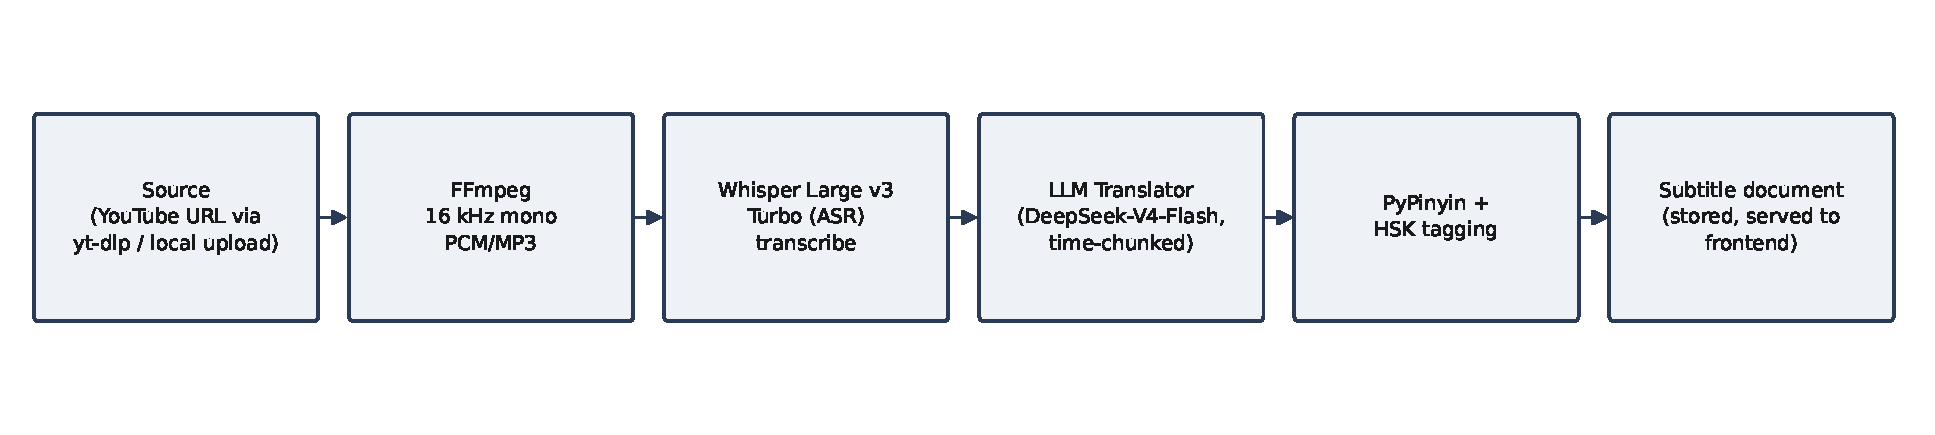
\includegraphics[width=0.95\textwidth]{./figs/fig_media_pipeline.pdf}
    \caption{Pipe and Filter realisation of the media-processing pipeline}\label{fig:media_pipeline}
\end{figure} Figure~\ref{lst:pipeline} shows the orchestrator that wires these filters together. Every step reports its own progress and elapsed time on its own, and if one step fails, none of the other filters need to know why --- they just don't receive any input. \begin{figure}[H]
\begin{verbatim}
async def run_pipeline(job_id, url, is_local=False):
    # 1. Download (yt-dlp) or accept local upload
    file_path = await asyncio.to_thread(download_video, url, job_id)

    # 2. Transcribe (Whisper Large v3 Turbo, FFmpeg-normalised audio)
    transcription = await asyncio.to_thread(api_transcribe, file_path)

    # 3. Translate (LLM, time-chunked) + pinyin/HSK annotation
    translation = await asyncio.to_thread(api_translate, transcription)

    # 4. Post-process into the final subtitle document shape
    end_result = await asyncio.to_thread(api_postprocess, translation)
\end{verbatim}
\caption{Simplified pipeline orchestrator (\texttt{backend-fastapi/api.py})}\label{lst:pipeline}
\end{figure} Each filter can be swapped out on its own. The transcription filter, for example, was moved from a locally-hosted Whisper model over to a cloud Whisper API midway through development, and nothing before or after it had to change, since the contract between stages --- a list of timestamped text segments --- stayed the same throughout.
\section{Core Feature: Generate Subtitles (UC06)}Subtitle generation is the entry point to every other feature in LexiFlow. When a video gets submitted, the \textbf{Whisper Large v3 Turbo} automatic speech recognition model transcribes it, a chat-completion language model translates it sentence-by-sentence into English, and then \textbf{PyPinyin} adds tone-marked pinyin along with per-character HSK difficulty levels. Figure~\ref{lst:translate} shows the translation filter. Segments get batched into five-minute time windows, which gives the model cross-sentence context without risking a truncated response, and the model has to return one JSON translation per input sentence, in order. \begin{figure}[H]
\begin{verbatim}
SYSTEM_PROMPT = (
    "...Respond with a JSON object of the exact form "
    '{{"translations": ["...", ...]}} containing exactly '
    "{count} strings, in the same order as the input...")

for chunk in _chunk_by_time(segments, chunk_seconds=300):
    translations = _request_translations(chunk_texts, ...)
    for segment, translated_text in zip(chunk, translations):
        segment["translated_text"] = translated_text
\end{verbatim}
\caption{Simplified LLM translation filter (\texttt{backend-fastapi/src/llm/translator.py})}\label{lst:translate}
\end{figure} The subtitle that comes out gets rendered on the watch page as a bilingual, pinyin-annotated transcript synced to the video. And every Chinese token is individually tappable: tap a character or word and you get an instant CC-CEDICT dictionary lookup (Figure~\ref{fig:ss_subtitles}) without playback stopping, which directly fulfils Search Word Definition (UC08) and feeds Save Vocabulary (UC09). \begin{figure}[H]
    \centering
    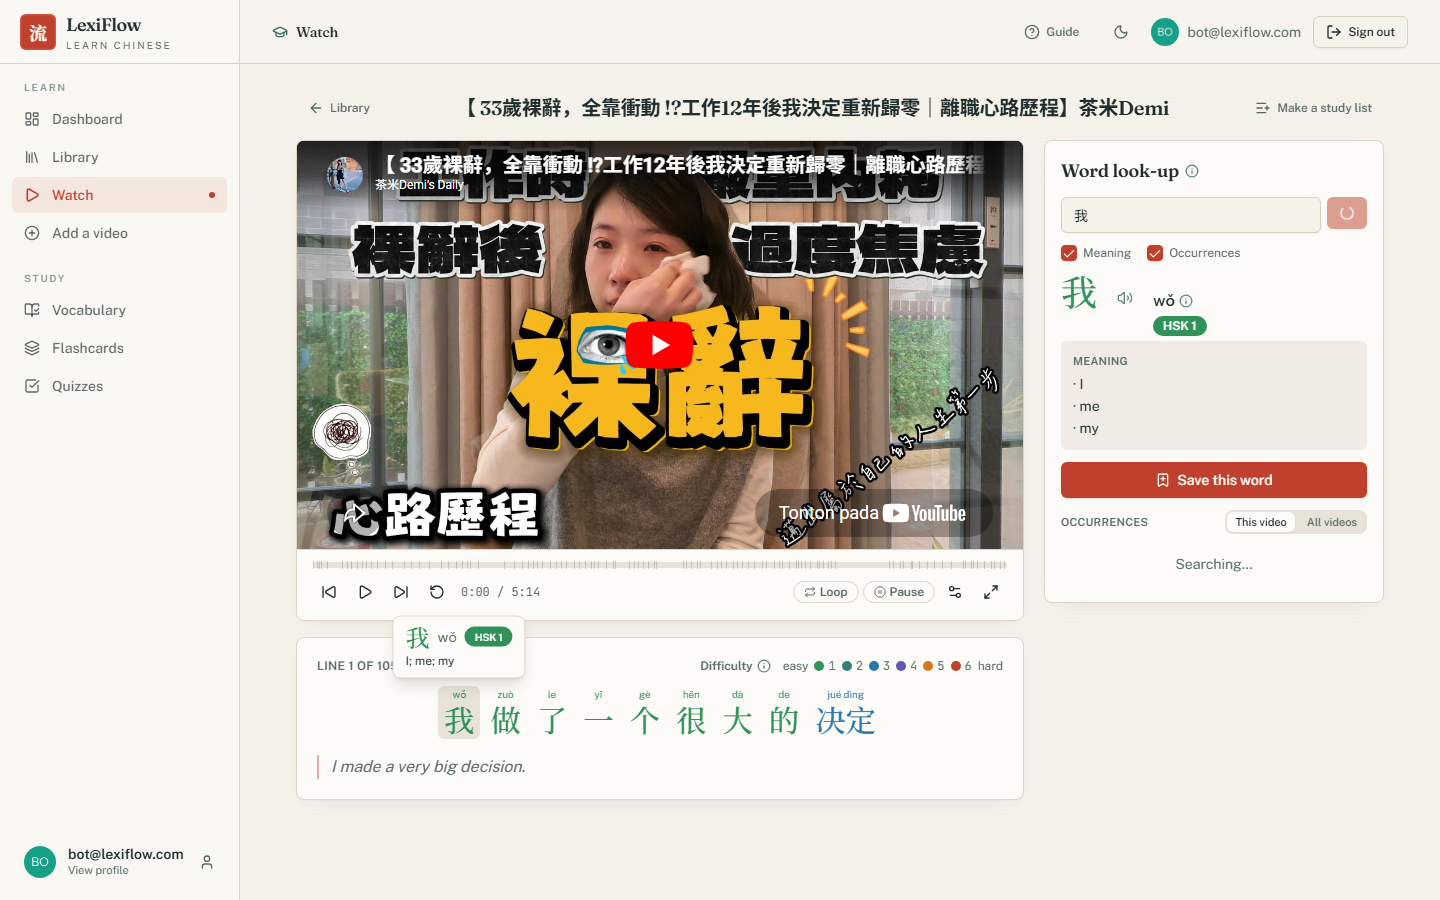
\includegraphics[width=0.7\textwidth]{./figs/fig_ss_subtitles.png}
    \caption{Bilingual subtitle playback with tap-to-look-up dictionary panel}\label{fig:ss_subtitles}
\end{figure}
\section{Core Feature: Generate and Review Flashcards (UC13)}Saved vocabulary gets reinforced through a spaced-repetition flashcard system built on the \textbf{FSRS (Free Spaced Repetition Scheduler) algorithm}, the same model behind the modern Anki ecosystem. Figure~\ref{fig:fsrs_growth} shows how the scheduled gap for a single item stretches out across successful reviews. Early ones sit a day or two apart. Items you've got down get pushed weeks into the future, so review effort lands where it actually matters. \begin{figure}[H]
    \centering
    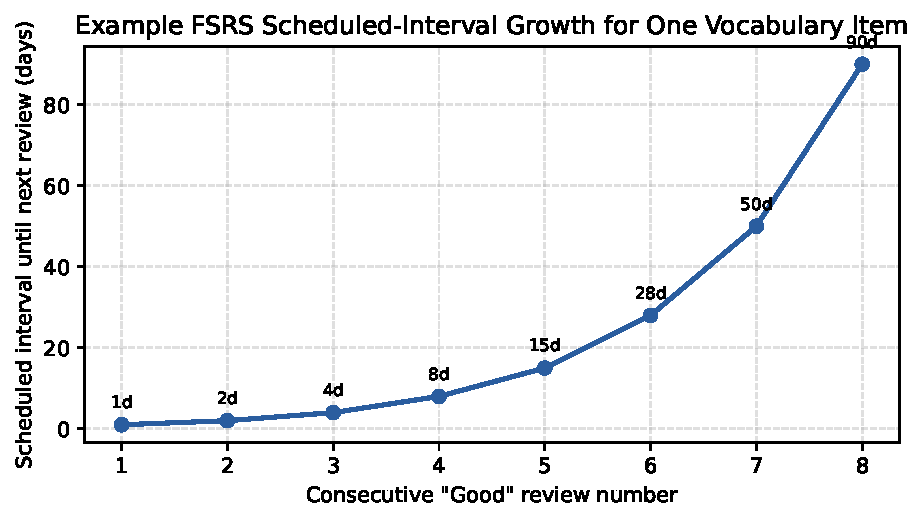
\includegraphics[width=0.7\textwidth]{./figs/fig_fsrs_growth.pdf}
    \caption{Example FSRS scheduled-interval growth for one vocabulary item}\label{fig:fsrs_growth}
\end{figure} Figure~\ref{lst:fsrs} shows the core scheduling function. Each grade (Again/Hard/Good/Easy) recomputes the item's Stability and Difficulty, then works out the next review date straight from the published FSRS weight parameters. We built this in-house rather than leaning on a third-party scheduling service. \begin{figure}[H]
\begin{verbatim}
function calculateFsrs(card, rating) {
    let { stability, difficulty, state } = card;
    if (card.state === 0 || stability === 0) {
        difficulty = clamp(FSRS_W[4] - FSRS_W[5] * (rating - 3), 1, 10);
        stability  = rating === 1
            ? FSRS_W[0]
            : FSRS_W[1] + FSRS_W[2] * (rating - 2)
                + FSRS_W[3] * Math.pow(rating - 1, 0.5);
    } else {
        const r = Math.pow(1 + 0.1 * (card.elapsedDays / stability), -1);
        difficulty = clamp(difficulty - FSRS_W[6] * (rating - 3), 1, 10);
        stability = /* FSRS stability-growth formula, rating-dependent */ ...;
    }
    const scheduledDays = clamp(Math.round(stability), 1, 365);
    return { stability, difficulty, scheduledDays, nextReviewDate: ... };
}
\end{verbatim}
\caption{Simplified FSRS scheduler (\texttt{backend-node/.../flashcards.service.js})}\label{lst:fsrs}
\end{figure} The frontend shows this as a flip-style card. The front displays only the Chinese word, and flipping it reveals pinyin and meaning next to the four grading buttons, each labelled with its resulting interval (Figure~\ref{fig:ss_flashcards}) so the learner sees the consequence of their self-assessment right away. \begin{figure}[H]
    \centering
    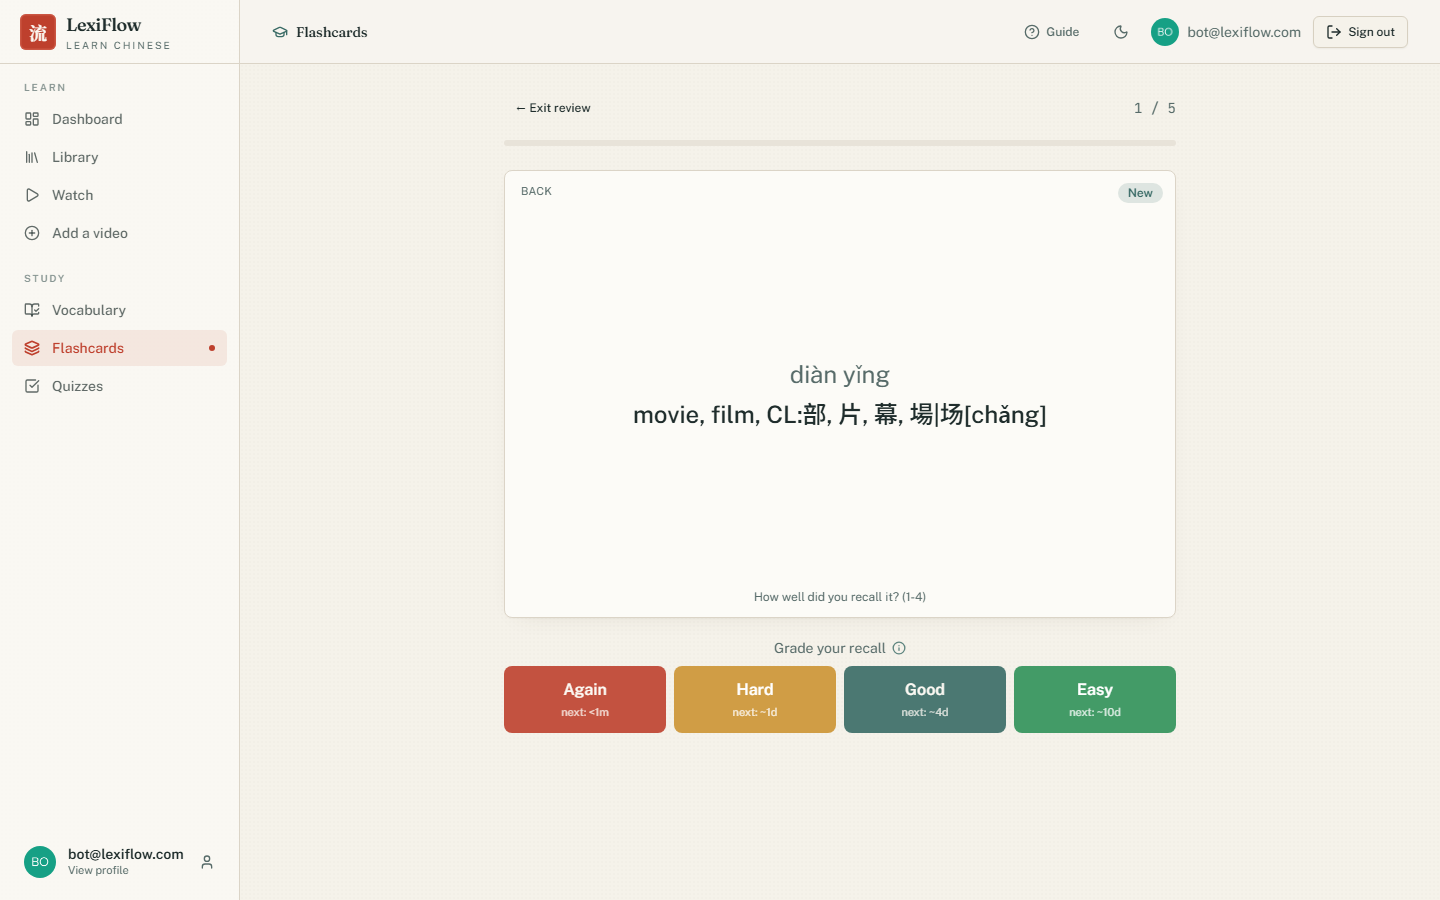
\includegraphics[width=0.7\textwidth]{./figs/fig_ss_flashcards.png}
    \caption{Flashcard review: back face with recall grading buttons}\label{fig:ss_flashcards}
\end{figure}
\section{Core Feature: Generate Quizzes (UC14)}LexiFlow can whip up a quiz on the fly from any vocabulary list, blending four question types: multiple choice, fill-in-the-blank, true/false, and short answer (Figure~\ref{fig:ss_quizzes}). For fill-in-the-blank, it just masks the target word inside a saved example sentence. Multiple-choice and true/false need something extra, though, plausible wrong answers, the distractors. \begin{figure}[H]
    \centering
    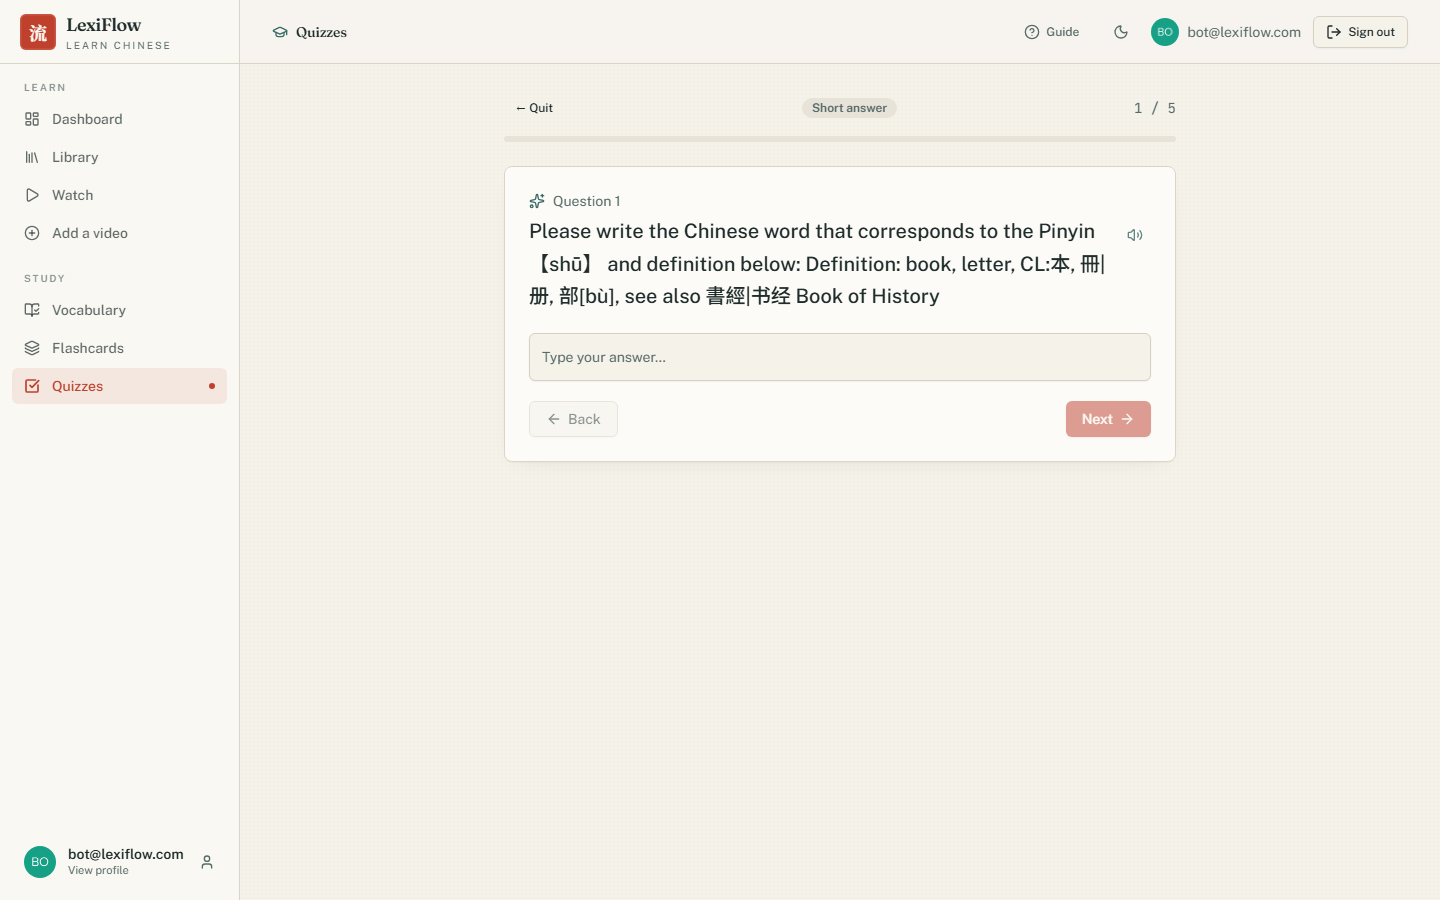
\includegraphics[width=0.7\textwidth]{./figs/fig_ss_quizzes.png}
    \caption{A generated short-answer quiz question}\label{fig:ss_quizzes}
\end{figure} Short-answer responses are trickier. You can't grade them by exact string matching, since one correct answer might be worded a dozen different ways. Figure~\ref{lst:judge} shows the grading filter: an exact match short-circuits right away, and if not, the reference answer and the learner's response both go to an LLM, which has to hand back a structured verdict. \begin{figure}[H]
\begin{verbatim}
def evaluate_short_answer(self, correct_reference, user_response):
    if ref_clean == resp_clean:
        return {"score": 1.0, "feedback": "Exact", "is_correct": True}

    content = self.provider.chat_complete(
        system=SYSTEM_PROMPT, user=json.dumps({...}), json_mode=True)
    result = json.loads(content)
    return {"score": result["score"], "feedback": result["feedback"],
            "is_correct": result["is_correct"]}
\end{verbatim}
\caption{Simplified short-answer judge (\texttt{backend-fastapi/services/quiz/judge.py})}\label{lst:judge}
\end{figure} Picking distractors for multiple-choice mixes that same LLM-based plausibility check with two light local heuristics: a pinyin Levenshtein-distance score (catching words that sound alike) and a radical/Unicode similarity score (catching ones that look alike). The three scores get summed, then the top candidates from the same HSK tier win out, so a distractor stays believable without ever sneaking in as an accidental synonym of the right answer.
\section{Core Feature: Crowd-Reporting of Translation Errors (UC11)}Anyone watching can flag a subtitle line as wrong, picking a category --- translation, pinyin, transcription, or other (Figure~\ref{fig:ss_crowdreport}). Plus but a line only gets bumped up for correction after it clears a deliberately cautious double threshold (Figure~\ref{lst:flag}): at least three different reporters, \emph{and} at least 25\% of everyone who actually saw that line. So one annoyed viewer can't flag stuff on their own. \begin{figure}[H]
    \centering
    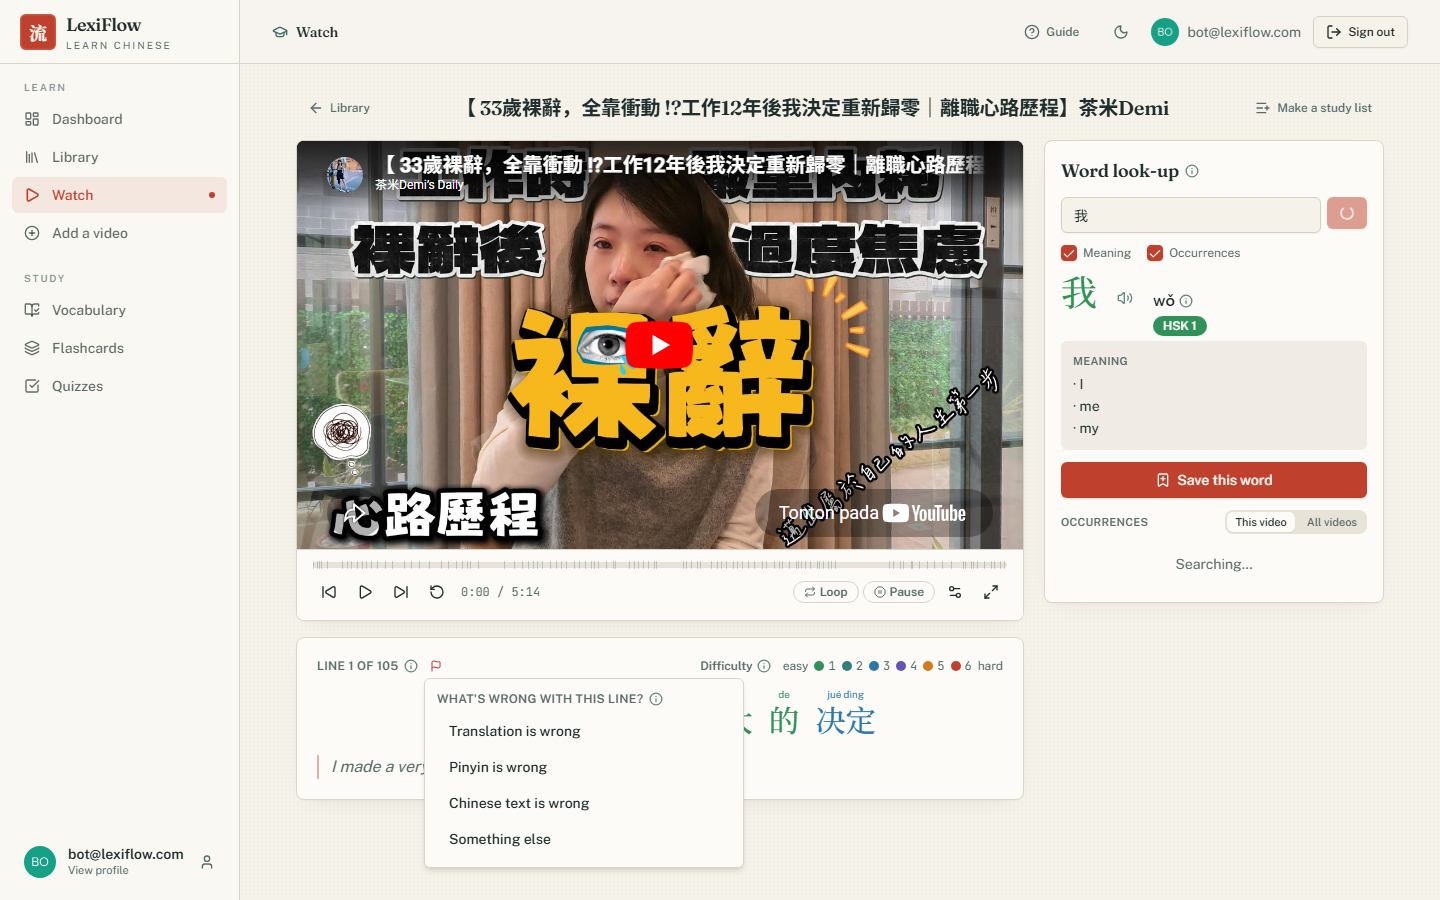
\includegraphics[width=0.7\textwidth]{./figs/fig_ss_crowdreport.png}
    \caption{Reporting a subtitle line and choosing an error category}\label{fig:ss_crowdreport}
\end{figure} \begin{figure}[H]
\begin{verbatim}
const FLAG_MIN_REPORTS = 3;
const FLAG_THRESHOLD_PERCENT = 0.25;
...
flagged: c.count >= FLAG_MIN_REPORTS
      && (c.count / viewerCount) >= FLAG_THRESHOLD_PERCENT
\end{verbatim}
\caption{Simplified flag threshold (\texttt{backend-node/.../reports.service.js})}\label{lst:flag}
\end{figure} Once it's flagged, the line gets fixed right away instead of sitting in a queue for a human moderator. The reported segment, three segments of surrounding context, and an instruction tied to the specific error category all get sent to \textbf{Meta's Llama 3.3 70B} model, which is locked to JSON-mode output. Here's the thing --- the original timestamps are always re-applied server-side rather than trusted to the model, so a hallucinated value can't ever knock the subtitle out of sync with the audio, and the fix is saved as a separate, reversible patch instead of overwriting the original transcription.
\section{Core Feature: Browser Extension}Want LexiFlow's bilingual subtitles on stuff you're already watching? A companion browser extension drops graded Chinese subtitles, word lookup, and text-to-speech right onto the YouTube player. No more copying video URLs into the main platform first. \begin{figure}[H]
    \centering
    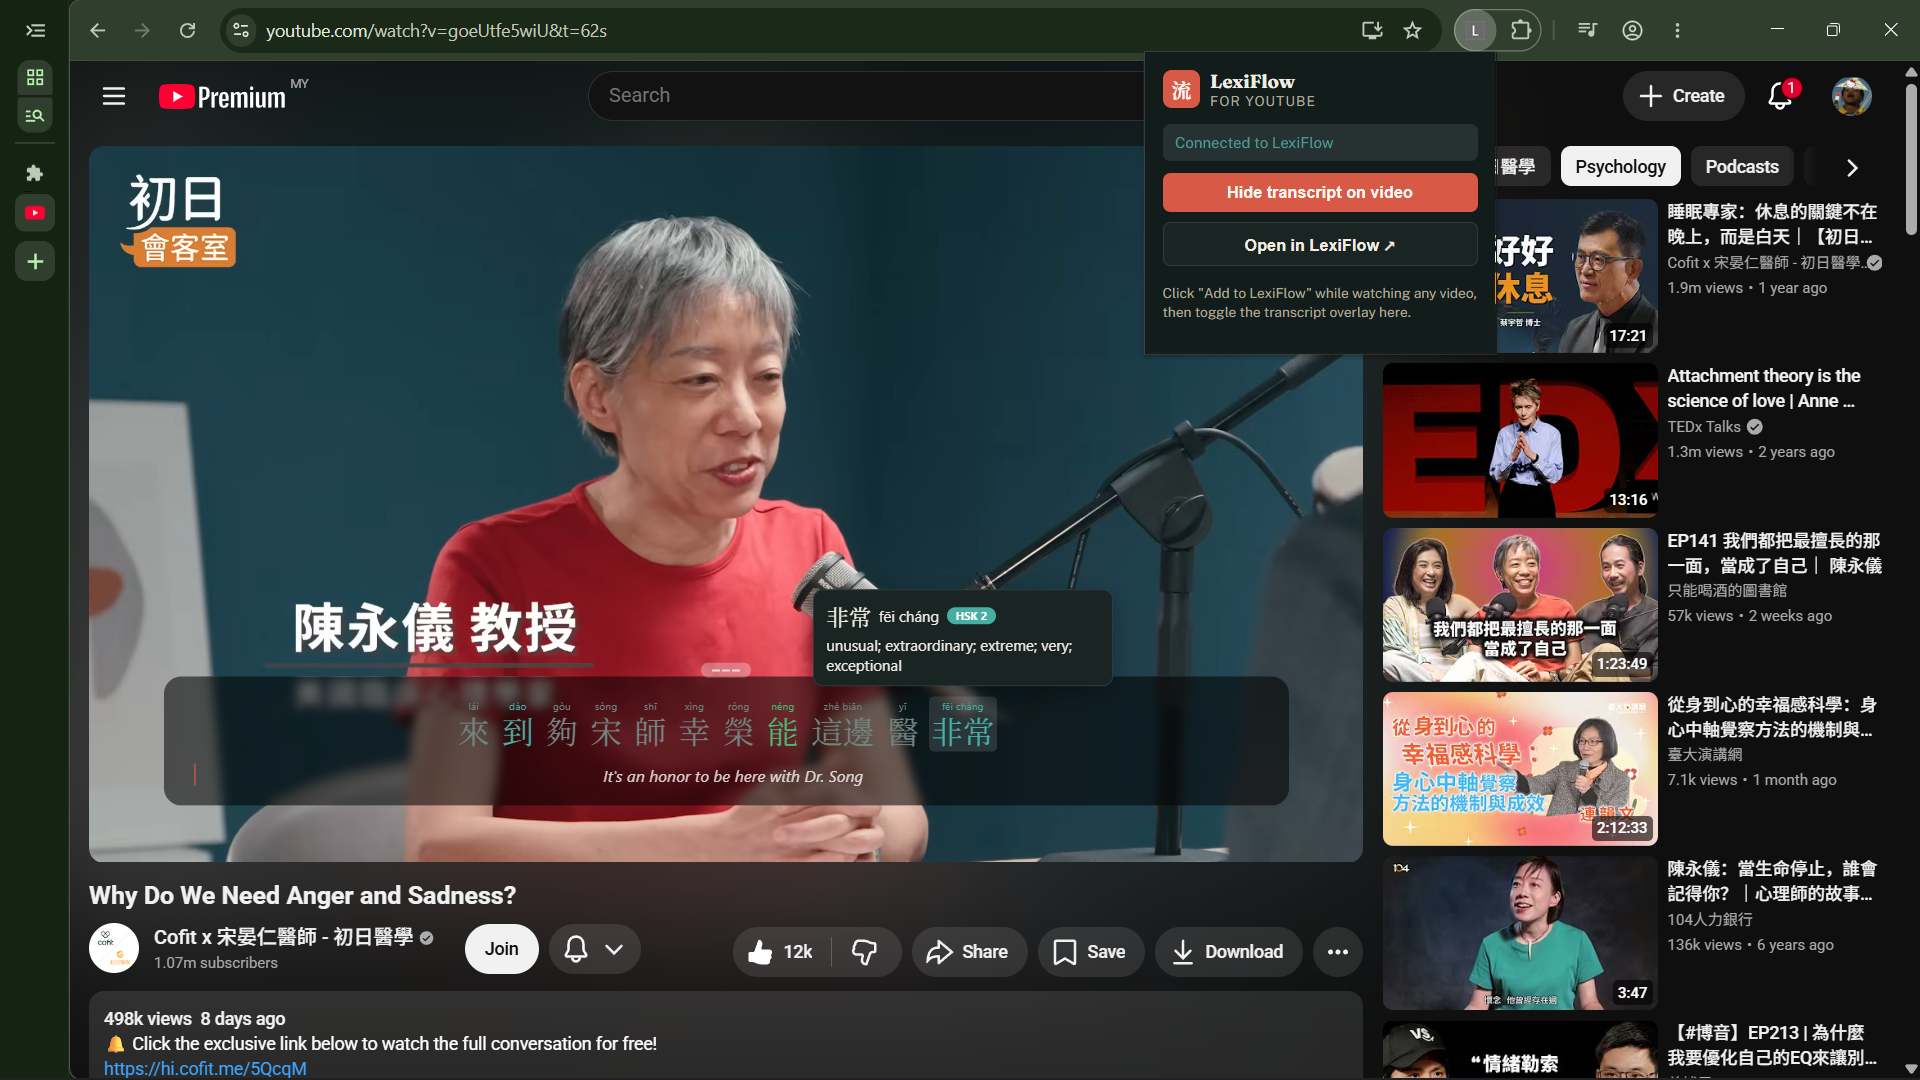
\includegraphics[width=0.95\textwidth]{./figs/fig_browser_extension.png}
    \caption{LexiFlow browser extension overlay on YouTube}\label{fig:ss_extension}
\end{figure}
\section{DevOps and Deployment}Figure~\ref{fig:deployment_topology} lays out where each piece of the system actually lives. But the frontend's a static build, served off \textbf{Vercel}'s edge CDN. The Node.js backend, the FastAPI worker, and PostgreSQL all sit together on one \textbf{Tencent Cloud Lighthouse} VM through Docker Compose, with a \textbf{SaladPool} instance kept around as a rarely-touched failover worker. On every push to \texttt{main}, \textbf{GitHub Actions} builds and pushes a container image to GHCR, then redeploys the VM on its own---so there's no manual deployment step. All AI inference---transcription, translation, quiz grading, segment correction---gets handed off to externally hosted language models (Whisper Large v3 Turbo, DeepSeek-V4-Flash, and Llama 3.3 70B), which means the deployment needs no GPU. \begin{figure}[H]
    \centering
    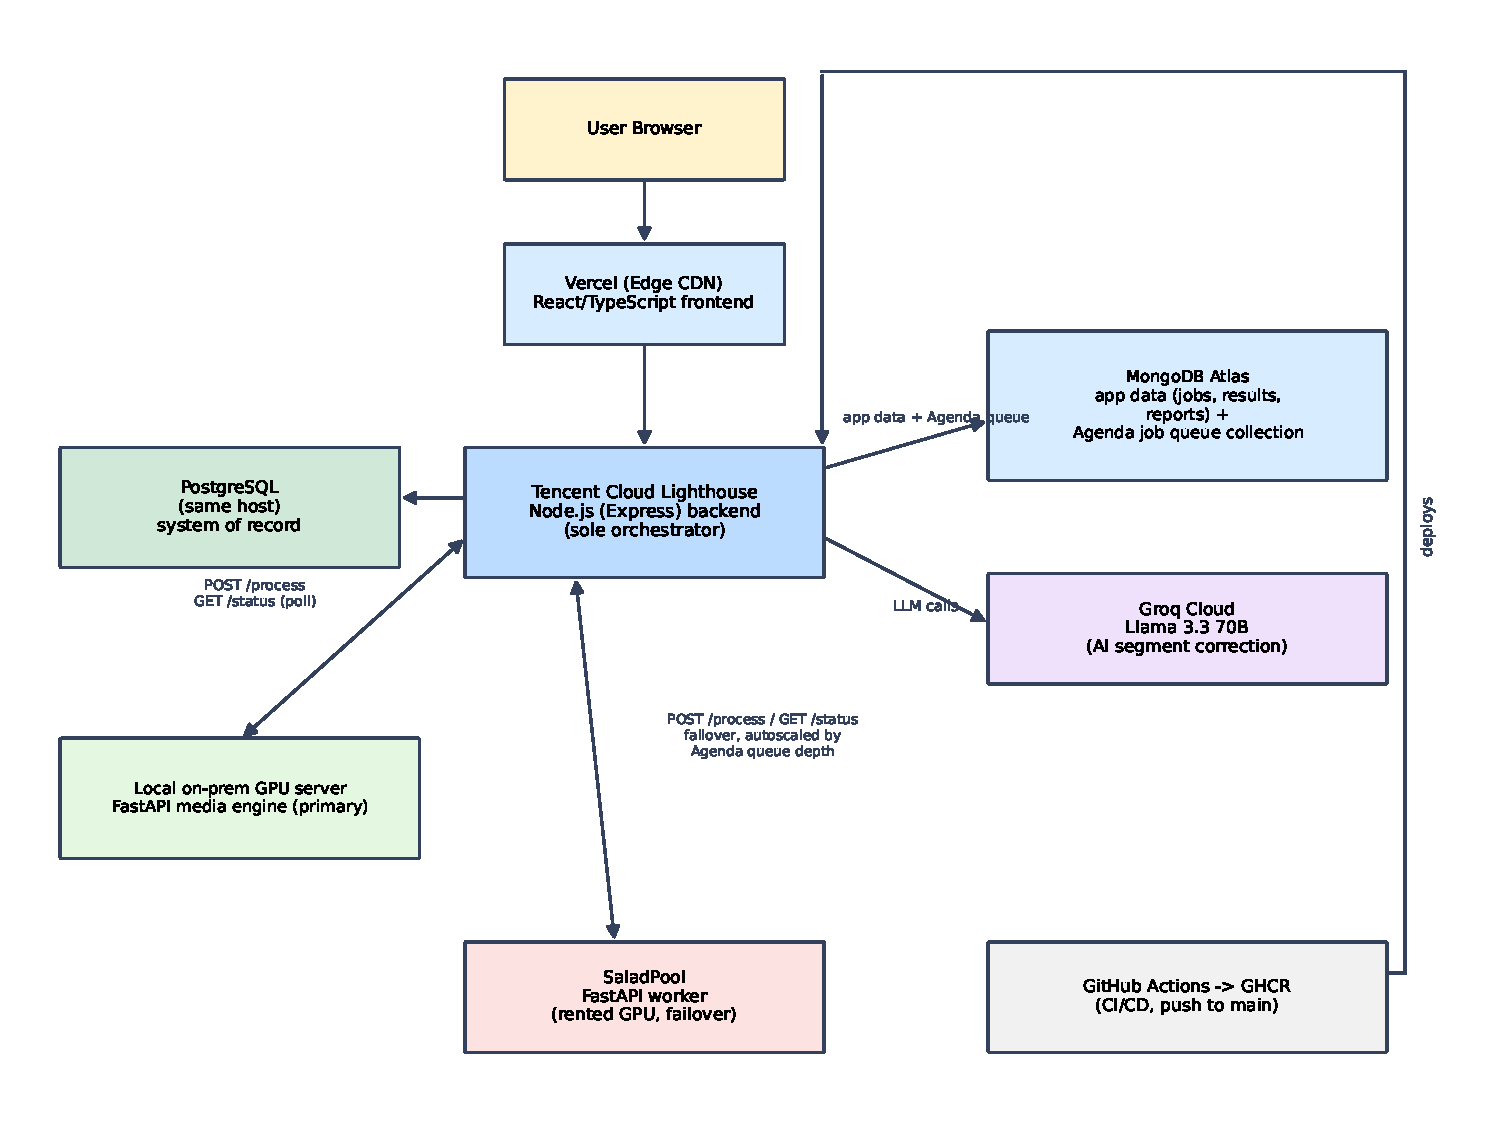
\includegraphics[width=0.95\textwidth]{./figs/fig_deployment_topology.pdf}
    \caption{LexiFlow deployment topology}\label{fig:deployment_topology}
\end{figure}
\section{Verification and Validation}We checked the system two different ways. First up, an automated end-to-end Playwright suite ran straight against the live test deployment, covering UC01 through UC14. Out of 30 test cases that gave us 25 passes, 4 failures, and 1 documented skip. The 4 failures came from two real, reproducible defects, an onboarding tour you couldn't dismiss and a missing single-page-application fallback route, not from anything wrong with the test scripts. Appendix~\ref{app:test-execution-report} lays out the full methodology, per-test-case results, and root-cause analysis. Then came User Acceptance Testing, run with four participants drawn from the user groups named in Chapter 4: a Mandarin learner who'd been struggling, a self-directed learner needing domain-specific vocabulary, a native-speaker reviewer checking transcription and translation accuracy, and the instructor stakeholder. Their feedback backed the value of the tap-to-look-up, vocabulary-saving, and quiz-generation flow. It also turned up two honest issues for later: an accuracy gap against commercial-grade captioning, and no classroom-management features, neither of which was scoped as a functional requirement back in Chapter 4. Full participant profiles, scenarios, and acceptance-criteria analysis sit in Appendix~\ref{app:uat-report}.
\section{Chapter Summary}So this chapter walked through how the Pipe and Filter architecture from Chapter 4 ended up as a pipeline you can swap out independently, then dug into the four core learning features --- subtitle generation, flashcards, quizzes, and crowd-sourced correction. Each one pairs a deterministic local algorithm (FSRS, threshold checks, pinyin/visual similarity) with an LLM only where open-ended judgement actually matters. Deployment stayed light on purpose; all the AI inference got handed off to external APIs. We verified the whole item through automated end-to-end testing plus User Acceptance Testing, and every defect we turned up traced back to a specific, reproducible root cause --- not some architectural flaw.
